\documentclass[a4paper,12pt]{article}

\usepackage{geometry}
\usepackage{fontspec}
\usepackage{ctex}
\usepackage{booktabs}
\usepackage{array}
\usepackage{tikz}

% Page setup with adequate margins
\geometry{
  a4paper,
  margin=2cm
}

% Set fonts
\setCJKmainfont{Kaiti TC}
\newCJKfontfamily\hanwangfont{HanWangKaiMediumChuIn} % HanWang font for Chinese headings

% Custom column types
\newcolumntype{C}{>{\centering\arraybackslash}m{1.5cm}}
\newcolumntype{D}{>{\centering\arraybackslash}m{1.2cm}}

% Custom command for large Zhuyin characters
\newcommand{\largezhuyin}[1]{{\fontsize{18pt}{22pt}\selectfont #1}}

% Custom command for large heading characters
\newcommand{\largehanzi}[1]{{\hanwangfont\fontsize{22pt}{26pt}\selectfont #1}}

\begin{document}

\begin{center}
\Large\textbf{\largehanzi{注音符號} Zhuyin Fuhao}
\end{center}

\vspace{0.5cm}

% CONSONANTS - Simple clean table
\noindent\textbf{\largehanzi{聲母} Consonants}

\vspace{0.2cm}
\begin{center}
\renewcommand{\arraystretch}{1.5}
\begin{tabular}{*{8}{D}}
\toprule
\largezhuyin{ㄅ} & \largezhuyin{ㄆ} & \largezhuyin{ㄇ} & \largezhuyin{ㄈ} & \largezhuyin{ㄉ} & \largezhuyin{ㄊ} & \largezhuyin{ㄋ} & \largezhuyin{ㄌ} \\
b & p & m & f & d & t & n & l \\
\midrule
\largezhuyin{ㄍ} & \largezhuyin{ㄎ} & \largezhuyin{ㄏ} & \largezhuyin{ㄐ} & \largezhuyin{ㄑ} & \largezhuyin{ㄒ} & \largezhuyin{ㄓ} & \largezhuyin{ㄔ} \\
g & k & h & j & q & x & zh & ch \\
\midrule
\largezhuyin{ㄕ} & \largezhuyin{ㄖ} & \largezhuyin{ㄗ} & \largezhuyin{ㄘ} & \largezhuyin{ㄙ} & & & \\
sh & r & z & c & s & & & \\
\bottomrule
\end{tabular}
\end{center}

\vspace{0.7cm}

% VOWELS - Simple clean table
\noindent\textbf{\largehanzi{韻母} Vowels}

\vspace{0.2cm}
\begin{center}
\renewcommand{\arraystretch}{1.5}
\begin{tabular}{*{8}{D}}
\toprule
\largezhuyin{ㄚ} & \largezhuyin{ㄛ} & \largezhuyin{ㄜ} & \largezhuyin{ㄝ} & \largezhuyin{ㄞ} & \largezhuyin{ㄟ} & \largezhuyin{ㄠ} & \largezhuyin{ㄡ} \\
a & o & e & ê & ai & ei & ao & ou \\
\midrule
\largezhuyin{ㄢ} & \largezhuyin{ㄣ} & \largezhuyin{ㄤ} & \largezhuyin{ㄥ} & \largezhuyin{ㄦ} & \largezhuyin{ㄧ} & \largezhuyin{ㄨ} & \largezhuyin{ㄩ} \\
an & en & ang & eng & er & i/yi & u/wu & ü/yu \\
\bottomrule
\end{tabular}
\end{center}

\vspace{0.7cm}

% TONES - Using TikZ for drawing tone marks
\noindent\textbf{\largehanzi{聲調} Tones}

\vspace{0.2cm}
\begin{center}
\renewcommand{\arraystretch}{1.8}
\begin{tabular}{*{5}{D}}
\toprule
\largehanzi{第一聲} & \largehanzi{第二聲} & \largehanzi{第三聲} & \largehanzi{第四聲} & \largehanzi{輕聲} \\
\midrule
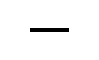
\begin{tikzpicture}
\draw[line width=1.5pt] (0,0) -- (0.5,0);
\end{tikzpicture} &

\begin{tikzpicture}
\draw[line width=1.5pt] (0,0) -- (0.5,0.3);
\end{tikzpicture} &

\begin{tikzpicture}
\draw[line width=1.5pt] (0,0.15) -- (0.25,-0.1) -- (0.5,0.3);
\end{tikzpicture} &

\begin{tikzpicture}
\draw[line width=1.5pt] (0,0.3) -- (0.5,-0.1);
\end{tikzpicture} &

\begin{tikzpicture}
\filldraw (0.25,0.1) circle (0.07cm);
\end{tikzpicture} \\
\bottomrule
\end{tabular}
\end{center}

\end{document}